% 1_introduction.tex

\cleardoublepage
\chapter{Introduction}
\textcolor{red}{I need to make it really clear that this work essentially sits before a detailed design optimisation, determining and analysis the mission profile in order to make informed decisions in the next design iterations}
  	
  	\textcolor{red}{I should make a point that the sensitivity analysis is a significant contribution}
  	
  	In recent years, the space sector has seen a significant shift in the paradigm of space launch system design. 
  	The sector has moved towards privatisation, with new and innovative launch systems competing to offer the most cost-efficient and reliable launches. 
  	The sector has also seen a split between those who produce large satellite launchers and those who produce small satellite launchers.
  	For large payload launchers, reusability is a major focus in the design of new launch systems, with the purpose of making a launch system cost efficient over multiple launches\cite{Faa2018}. 
  	For small payload launchers, reusability is more complex than for large launchers, as the additional systems necessary for reusability add a larger fraction of system mass, and require a proportionally larger fuel mass. 
  	Consequently, the focus of small launch system design is currently on producing expendable launch systems as cheaply and efficiently as possible, using state of the art technologies such as 3D printing to expedite the process and minimise cost\cite{Niederstrasser2015}.
  	However, if reusability is able to be successfully integrated into small launch system design, it has the potential to increase the cost efficiency and launch flexibility, potentially opening up the small satellite market significantly. 
  	
  	
  	
  	A potential candidate for integrating reusability into small satellite launch systems is the use of airbreathing engines\cite{Smart2009a,Ketsdever2010}.
Airbreathing engines produce higher specific impulse than rockets, and do not require oxidiser to be carried on-board a launch vehicle\cite{Smart2010}.  	 
  	The higher efficiency and reduced propellant mass of airbreathing vehicles allows the additional mass of the systems necessary for reusability to be mitigated\cite{Curran2003}. An airbreathing vehicle can be designed in a similar fashion to a conventional aircraft, with wings, stabilisers and ailerons\cite{Shaughnessy1990,Preller2017b}. A vehicle designed in this fashion has a high lift-to-drag ratio, and good manoeuvrability, allowing for a return flight and landing on a conventional landing strip\cite{Preller2017b}. This style of return removes the need for transport, enabling a fast turn-around and cost-efficient re-use. 
  	
  	The primary airbreathing engines in consideration for launch vehicles are ramjet and scramjet engines\cite{HeiserWilliamPratt1994}. These engines offer good efficiency and have operational regimes that allow them to effectively accelerate a launch vehicle over a range of Mach numbers. 
  	Ramjets and scramjets rely on the high velocity of the aircraft to compress the flow of air entering the engine before combustion.  Ramjets slow the air to subsonic speeds before combustion and are limited to operation at low Mach numbers, whereas scramjets keep the flow supersonic throughout, and operate within the hypersonic regime, above Mach 5. 
  	These engines have limited operational regimes, and require atmospheric flight in order to take oxidiser from the air. These operational constraints mean that a launch system cannot be solely powered by airbreathing engines. Rocket power is necessary for at least the exoatmospheric portion of the trajectory. As a result, the designs of airbreathing launch systems require rocket stages, usually separated into multiple stages to increase weight efficiency\cite{Smart2009a}. If a scramjet engine is used as the airbreathing engine of the launch system, rocket power is also desirable for accelerating scramjet accelerator to minimum operational speed, as the alternative is using turbojets and ramjets sequentially\cite{Smart2009a}, which is weight and cost intensive. 
  	
  	 
  	 
  	 Calculating a suitable trajectory for an airbreathing launch system is an integral part of the preliminary vehicle and mission design process. 
  	 A trajectory must be calculated that allows the launch system to achieve its objective of placing a payload into orbit, while recovering any reusable stages.
  	 Ideally, the calculated trajectory will achieve the maximum possible payload-to-orbit, while adhering to the structural, heating and propulsive limitations of the vehicle.  
  	 The trajectory design for a partially-airbreathing launch system is complex and requires consideration of each of the individual stages in order to maximise the performance of the launch system, and consequently, its cost efficiency. 
  	   The airbreathing engines of a ramjet or scramjet-powered stage require high dynamic pressure to operate effectively, and airbreathing stages are generally designed for high lift-to-drag. Conversely, rocket-powered stages operate more efficiently at higher altitude, and are generally designed for weight and cost efficiency. For these launch systems, the various stages and engines involved during launch require trade-offs in engine efficiency and thrust generation, stage mass, and vehicle aerodynamics. These factors require the launch trajectory of the system to be thoroughly simulated and optimised, to ensure that the launch vehicle is operating effectively. 
  
    Optimal control theory is a general set of techniques which find a control law to maximise a given metric of a system, subject to a set of constraints\cite{Rao2009,Betts1998}. 
    Optimal control theory can be used to calculate the optimised trajectory profile for a launch vehicle in a robust and computationally efficient manner, allowing a trajectory to be calculated in which the flight path of each individual stage is considered simultaneously to produce a maximum-payload trajectory\cite{Betts1998}. 
  Optimal control is able to produce an optimised trajectory which satisfies the specific structural and flight constraints of the vehicle being simulated, allowing the physical limitations of the vehicle, such as heating and structural loading limits, to be imposed\cite{Betts1998}. These constraints also allow any necessary mission conditions to be established, such as reaching orbital velocity and achieving fly-back. 
  An optimal trajectory calculated for multiple launch vehicle stages simultaneously, without predispositions, can offer valuable insights into the performance of a launch vehicle, and drive future design decisions. 
  This concurrent optimisation of multiple stages is particularly important for launch systems incorporating airbreathing engines, where the performance and operational requirements of each stage are significantly different.  
  



  
  
  	   This study applies optimal control theory to a three stage rocket-scramjet-rocket launch system being developed by The University of Queensland, The second stage of this system is a scramjet-powered accelerator, designated the SPARTAN\cite{Preller2017b}. This launch system is designed to be partially reusable, with at least the second stage scramjet vehicle flying back to the initial launch site, as well as possibly the first stage booster\cite{Preller2017b} although this is beyond the scope of this study. 
  	   In previous studies it has been assumed that by maximising the performance of the SPARTAN, that the performance of the launch system is also maximised\cite{Preller2017b}. 
  	   The trajectory of the launch system has been designed around the SPARTAN flying at its
  	   maximum dynamic pressure, and all other trajectory stages have conformed to this assumption. However, these studies did not consider the interaction between stages, or the fly-back of the SPARTAN.
  	   This study will develop trajectory planning tools for partially-airbreathing launch systems, and calculate an optimised launch trajectory for the rocket-scramjet-rocket system incorporating the SPARTAN. This optimised trajectory will be calculated with the aim of producing an optimal
  	   trajectory profile which may be applied to any multi-stage rocket-airbreathing-rocket system for delivering small
  	   satellites to Earth orbit. The impact of the fly-back of the scramjet stage on the optimised trajectory will be studied, and the ability of the rocket-scramjet-rocket system to effectively deliver small payloads to orbit and return the scramjet stage to its initial launch site will be assessed. 
  	   
  	  	\begin{figure}[ht]
  	  		\centering
  	  		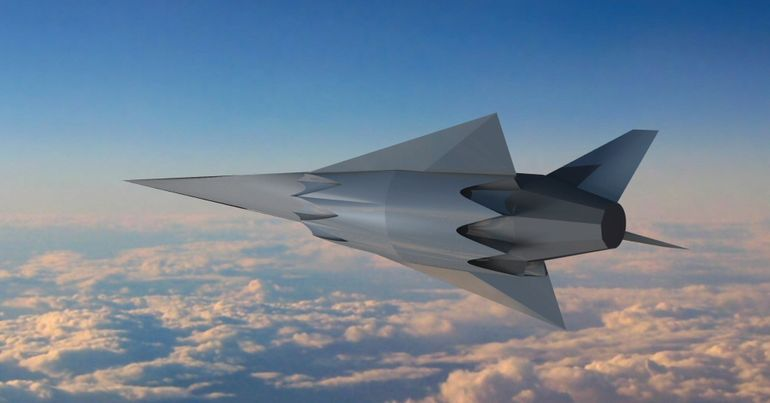
\includegraphics[width=0.7\linewidth]{figures/1_introduction/project-spartan}
  	  		\caption{The SPARTAN scramjet-powered accelerator\cite{BBC}.}
  	  		\label{fig:project-spartan}
  	  	\end{figure}
  	  	

  \section{Research aims}

    The aim of this work is to design the trajectory of a rocket-scramjet-rocket small satellite launch system. The purpose of this optimised trajectory is to maximise the payload-to-orbit capabilities of the launch system, thereby also maximising the cost efficiency of the system. The optimal trajectory will be utilised to assess the feasibility of return flight, as well as to determine the impact of key vehicle design parameters on the performance of the launch system. 
 
    
\vspace*{10pt}
    \noindent These aims will be achieved by addressing the following objectives:
    \begin{enumerate}
    	 \item \emph{Development of a detailed design and aerodynamic simulation for a rocket-scramjet-rocket launch system.}
    	 
    	   A detailed launch system design and robust dynamic simulation are required in order for optimal control to be applied to a launch system. The design must be representative of a standard rocket-scramjet-rocket launch system for the optimal trajectory results to be generally applicable. The dynamic simulation must be accurate and robust in order for the optimised trajectory to be meaningful. \\

\item \emph{Calculation of the maximum payload-to-orbit trajectory for a rocket-scramjet-rocket launch system using optimal control, with and without fly-back.}

The optimal trajectory shape of a multi-stage rocket-scramjet-rocket system is sensitive to the design and aerodynamic characteristics of each stage, and cannot be easily assumed. The use of optimal control techniques allows a maximum-payload trajectory to be calculated with few assumptions as to the general shape of the trajectory. The inclusion of the fly-back of the scramjet stage in the trajectory optimisation allows the impact of the fly-back to be minimised.\\

      \item \emph{Analysis of the sensitivity of the maximum payload-to-orbit trajectory to variations in key design parameters of the launch system} 

	The optimal trajectory shape and maximum payload-to-orbit are dependent on the design of the launch system. 
	Assessing the sensitivity of the optimised trajectory shape and payload-to-orbit to key aerodynamic and propulsive properties allows the relative impacts of various design parameters to be calculated and contrasted, and for the optimal trajectory shape to be investigated. \\

    

    \end{enumerate}

  \clearpage
  \section{Thesis Outline and Contributions}

    

    \subsubsection*{Chapter 2 - Literature Review}

      A review of literature related to the various aspects of this study is presented. The theory behind scramjet propulsion is outlined, followed by a background of reusable and small satellite launch systems. A review of the trajectories of partially-airbreathing launch systems is presented, comparing the optimised trajectories of various conceptual vehicles. An overview of optimal control techniques is presented, with particular emphasis on the pseudospectral method of solving optimal control problems, which is employed within this study. Lastly, an overview of the optimal control and aerodynamic solvers that are used in this study is presented.
      

    \subsubsection*{Chapter 3 - Launch Vehicle Design and Simulation}

      The design, aerodynamics and engine models of all three stages are detailed. The SPARTAN scramjet-powered stage is presented first, followed by the first and third stages. The design of each stage is shown, along with sizing and mass breakdowns. The propulsion model used for each stage is detailed, along with the modelling and interpolation schemes used. The aerodynamic characteristics and simulation methodology of each stage is presented, and the process for trimming each vehicle is specified. 
      
      
      \subsubsection*{Chapter 4 - LODESTAR}
      
      The method used for the simulation and optimisation of the trajectory is presented, including the details of the trajectory analysis program, LODESTAR, which has been developed for this study. The specifics of the optimal control methodology are presented. The simulation methodology is detailed, along with the construction of the optimal control simulation for the mission used in this study. The specific set-up of the optimal control program is detailed for each trajectory stage, specifying the costs and constraints which drive the optimal control solver. Finally, the methods for validating the final solutions are specified.
      
      \subsubsection*{Chapter 5 - Optimised Ascent Trajectory}
      
Optimised trajectories, designed using LODESTAR, are presented. A trajectory is designed in which the SPARTAN flies at a constant dynamic pressure, for comparison purposes. 
 A maximum payload-to-orbit trajectory is created and it is found that an increase in altitude at the stage separation points significantly improves payload-to-orbit.
 This trajectory is compared and contrasted to the constant dynamic pressure trajectory to determine the sources of the performance increase.  
 Key vehicle design parameters are varied. The trends in maximised payload-to-orbit and trajectory shape are analysed to study the relative impact of the design parameters on the performance of the launch system. 
 
 
      
      \subsubsection*{Chapter 6 - Optimised Trajectory Including Fly-Back}
      
      The trajectory of the launch system is optimised for maximum payload-to-orbit, including the fly-back of the SPARTAN to its initial launch location. 
      It is found to be necessary to reignite the scramjet engines during the return flight of the SPARTAN to achieve fly-back.
      The SPARTAN is found to bank during acceleration to lessen the fuel consumed during the return flight.
      The trajectories with, and without, fly-back are compared to determine the impact of SPARTAN fly-back on the performance of the launch system
      In a similar fashion to Chapter 5, the effects of key vehicle parameters on the optimised trajectory are studied. The sensitivity of the optimised trajectory and payload-to-orbit are analysed, with emphasis on how the fly-back trajectory is affected by the varied vehicle parameters.
      
     
      

    \subsubsection*{Conclusions and Recommendations}

      The body of this thesis concludes by summarising the most significant findings from this work. Recommendations for future work are made. 